\documentclass[]{article}

\usepackage{caption,subcaption,graphicx,float,url,amsmath,amssymb,amsthm,tocloft,cancel,thmtools,gensymb,braket}
\usepackage[toc,nonumberlist]{glossaries}
\usepackage{glossaries-extra}
\newcommand\numberthis{\addtocounter{equation}{1}\tag{\theequation}}
\newtheorem{defn}{Definition}
\newtheorem{thm}{Theorem}
\newtheorem{cor}[thm]{Corollary}
\newtheorem{lemma}[thm]{Lemma}
\graphicspath{{figs/}}
\widowpenalty10000
\clubpenalty10000

%opening
\title{Theoretical Minimum\\Advanced Quantum Mechanics}
\author{Simon Crase}

\begin{document}

\maketitle

\begin{abstract}
These are my notes from the Advanced Quantum Mechanics lectures from Leonard Susskind's Theoretical Minimum series.
\end{abstract}

\tableofcontents
\listoffigures

\section{Review and Introduction to Symmetry}

\subsection{Review of Quantum Mechanics}

\begin{itemize}
	\item States: $\ket{\Psi}$ and $\bra{\Psi}$
	\item Observables: $A=A^{\dag}$
	\item Eigenvalues represent values that can be measured: $A\ket{\alpha} = \alpha\ket{\alpha}$
	\item Inner product $\braket{\phi|\psi}$	
	\item Orthogonal $\braket{\phi|\psi}=0$
	\item Independent values $\braket{x|x^{\prime}}=0$
	\item Wave function $\braket{x|\psi} = \psi(x)$
	\item Probability $P(x)=\psi^*(x)\psi(x)$
	\item Momentum $p\psi(x)=- i \hslash \frac{\partial \Psi}{\partial x}$
	\item Evolution $U(t)-- \ket{\psi(0)} = \ket{\psi(t)}$
	\item $\braket{\phi|\psi}=\braket{\phi|U^{\dagger}U|\psi}$ i.e. $U^{\dagger}U=I$
	\item $U(\epsilon)= I + \epsilon G$, so $G=-G^{\dagger}$, $G=- i H$
	\item For general $t$, $U(t)=e^{- i H t}$
\end{itemize}

\begin{align*}
=& e^{-i \hslash \epsilon} \ket{\psi(t)}\\
=& (1- i \hslash \epsilon)\ket{\psi(t)}\\
\frac{\ket{\psi(t+\epsilon)} -\ket{\psi(t)} }{\epsilon}&= -i \hslash \ket{\psi(t)}\\
\frac{\partial \ket{\psi}}{\partial t} =& -i H \ket{\psi(t)} \text{, Time dependent Schr\"odinger Equation}\\
H \ket{\psi} =& E \ket{\psi}\text{, Time independent Schr\"odinger Equation}
\end{align*} 


\subsection{Introduction to Symmetry}

Rotational symmetry is one of the most important symmetries. So is translational symmetry. Transformation is a symmetry that doesn't change equations.

\begin{align*}
V \ket{\psi} =& \ket{\psi^{\prime}} \text{, symmetry operation -- unitary $V$}\\
\ket{\psi_1} \xrightarrow{U}& \ket{\psi_2} \text {, time evolution}\\
\ket{\psi_1^{\prime}} \xrightarrow{U}& \ket{\psi_2^{\prime}} \text {, if $V$ really is a symmetry. Now}\\
V\ket{\psi_2} =& U V \ket{\psi_1} \text{, and}\\
V U\ket {\psi_1} =& U V \ket{\psi_1} \\
V U =& U V \\
V H =& H V\\
[H,V] =& 0
\end{align*}

Symmetry is unitary operator that commutes with Hamiltonian.

\begin{itemize}
	\item Discrete
	\begin{itemize}
		\item Reflection
		\item interchange particles
	\end{itemize}
	\item Continuous
	\begin{itemize}
		\item rotation
		\item translation
	\end{itemize}
\end{itemize}

All continuous symmetries can be generated by $I-i \epsilon G$, for some Hermitean $G$ -- $[H,G]=0$.

E.g.
\begin{align*}
V \psi(x) = & \psi(x-\epsilon)\text{, shift right}\\
=& \psi(x) - \epsilon \frac{\partial \psi}{\partial x}\\
V =& I -  \epsilon \frac{\partial }{\partial x}\\
=& I - \frac{i \epsilon}{\hslash}P\\
G =& \frac{P_x}{\hslash}\text{, Generator of $x$ translation}
\end{align*}


\section{Symmetry groups and degeneracy}

Crystal symmetry: translate one lattice spacing.

Degeneracy of energy levels: more than one state with given energy. Only happens when there is a symmetry.

Rotation.

\begin{align*}
\psi(\theta) \rightarrow & \psi(\theta - \epsilon)\\
\delta\psi =& - \epsilon \frac{\partial \psi}{\partial \theta}\\
=& -i \epsilon \big(-i \frac{\partial \psi}{\partial \theta}\big).\text{ Now defining the Angular Momentum operator $L$}\\
- i \frac{\partial}{\partial \theta} =&\hslash L \\
\delta\psi =& - \frac{i \epsilon}{\hslash} L \psi \text{, generator of rotation}
\end{align*}

Eigenvalues and Eigenvectors.

\begin{align*}
L\ket{\psi} =& l \ket{\psi}\\
-i \hslash \frac{\partial \psi}{\partial \theta} =& \psi\\
\psi(\theta) =& e^{\frac{i m \theta}{\hslash}}\text{Now, we want $\psi$ single valued, so}\\
\frac{m}{\hslash}=&k\text{, some integer. But, by convention, redefine $m$}\\
L=& m \hslash
\end{align*}
This is the quantization of angular momentum.

$n\ne 0 \implies E(m)=E(-m)$, so we have degeneracy. A magnetic field breaks this; symmetry isn't enough for degeneracy, but adding reflection symmetry is sufficient (but need two non-commuting symmetries).

\begin{thm}[Reflection and rotation don't commute]
	If $M\psi(\theta) = \psi(-theta)$, $ML \ne LM$
\end{thm}
\begin{proof}
	\begin{align*}
	MLe^{i m \theta} =& M m e^{i m \theta}\\
	=&m e^{- i m \theta}\\
	LMe^{i m \theta} =& L e^{- i m \theta}\\
	=& -m e^{- i m \theta}
	\end{align*}
\end{proof}

\begin{align*}
[L,H]=& 0\\
[L_x,L_y] =& i L_z \numberthis \label{eq:lx_ly}\\
[L_y,L_z] =& i L_x\numberthis \label{eq:ly_lz}\\
[L_z,L_x] =& i L_y\numberthis \label{eq:lz_lx}\\
L_{\pm} \triangleq& L_x \pm i L_y\\
[L_{\pm},L_Z] =& \mp L_{\pm}
\end{align*}
Suppose we have found one eigenvector:
\begin{align*}
L_z \ket{m} =& m \ket{m}\\
[L_+,L_z] \ket{m} =& \big(L_+L_z - L_z,L_+\big) \ket{m}\\
=&- L_+ \ket{m}\\
 m L_+\ket{m} + L_+\ket{m} =& L_z L_+ \ket{m} \text{, whence}\\
 \big(m + 1 \big)L_+\ket{m}  =& L_z L_+ \ket{m} \text{, i.e. $L_+ \ket{m}$ is an eigenvector, eigenvalue $m+1$.}\numberthis \label{eq:create_m}
\end{align*}

Similarly, $L_- \ket{m}$ is an eigenvector, eigenvalue $m-1$. This terminates if  $L_{\pm} \ket{m}=0$. From symmetry we can show $m$ integral or half integral.

\begin{thm}[Eigenvectors have same energy.]
	 $H \ket{m} = E \ket{m} \implies H \ket{m \pm 1} = E \ket{m \pm 1}$
\end{thm} 
\begin{proof}
	\begin{align*}
	H \ket{m} =& E \ket{m}\\
	H L_+ \ket{m} =& L_+ H \ket{m}\\
	=& L_+ E \ket{m}\\
	H \ket{m+1} =& E \ket{m+1}
	\end{align*}
\end{proof}

Since symmetries commute, we have degeneracy.

\section{Atomic orbits and harmonic oscillators}

\subsection{Atomic orbits}

A particle moving in a central force field: angular momentum and orbital plane preserved. State is $\psi(r,\theta,\phi)= \psi(r,\theta)$, and $L = -i \frac{\partial}{\partial \theta}$.

\begin{align*}
-i \frac{\partial \psi(r,\theta)}{\partial \theta} =& l \psi(r,\theta) \text{, eigenvector}\\
\psi(r,\theta) =& e^{i l \theta} \chi(r) \text{, for some $\chi$}
\end{align*}
More generally, $\psi(r,\theta,\phi)= Y(\theta,\phi) \chi(r)$


From (\ref{eq:create_m}) we have a spectrum of angular momenta, integral or half integral, say $\set{-l,...,l:L_+\ket{l}=0}$. There are $2l+1$ states with constant $L^2 = L_x^2 + L_y^2 + L_x^2$. Classically $L^2 = L_z^2 +(L_x-iL_y)(L_x+iL_y)$, but this fails in quantum mechanics as they operators don't commute.

\begin{align*}
L^2 =& L_z^2 +(L_x-iL_y)(L_x+iL_y) -i [L_x,L_y]\\
=& L_z^2 + L_z + L^-L^+\\
L^2\ket{l}=& L_z^2\ket{l} + L_z\ket{l} + L^-L^+\ket{l}\\
=& l^2\ket{l} + l\ket{l} + 0\\
L^2\ket{l}=&l (l+1) \ket{l}
\end{align*}

\begin{thm}[All eigenvectors of $L_z$ are degenerate eigenvectors of $L^2$]
	\begin{enumerate}
		\item $[L^2, L_i] =0$
		\item All eigenvectors of $L_z$ are eigenvectors of $L^2$, eigenvalue $l(L+1)$
	\end{enumerate}
\end{thm}
\begin{proof}
	Exercise
\end{proof}

\begin{figure}[H]
	\caption{Degeneracy of Energy Levels in Hydrogen Atom}\label{fig:degeneracy:hydrogen}
	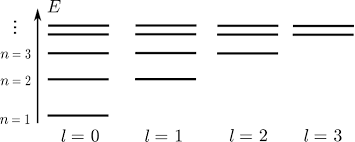
\includegraphics[width=0.9\textwidth]{hydrogen-degeneracy}
\end{figure}
Classically:
\begin{align*}
H =& \frac{p^2}{2m} + V(r) \text{, conserved} \numberthis \label{eq:classical:Hamiltonian}\\
L =& r \times P  \text{, conserved, so use xy plane}\\
H =& \frac{p_r^2+p_{\theta}^2}{2m} +V(r)\\
=& \frac{P_r^2}{2m} + \frac{L^2}{2m r^2} + V(r) 
\end{align*}

Schr\"odinger Equation:
\begin{align*}
-\frac{\hslash^2}{2m}\frac{\partial^2 \psi(r)}{\partial r^2} + \frac{l(l+1)\hslash^2}{r^2}\psi(r)+V(r)\psi(r) =& E\psi(r)\numberthis \label{eq:schroedinger:central}
\end{align*}

Number of nodes (zeroes) characterize energy levels.

Classical mechanics inspires choice of Hamiltonian(\ref{eq:classical:Hamiltonian}), but Schr\"odinger equation (\ref{eq:schroedinger:central}) is quantum.

\subsection{Harmonic oscillators}

Everything in physic that disturbs equilibrium by a small amount can be approximated by a simple harmonic oscillator. 

Start with suspended mass $(m=1)$, spring constant $(k=\omega^2)$

\begin{align*}
H =& \frac{P^2}{2m} + \frac{\omega^2 x^2}{2}\\
=& \frac{\omega}{2 \omega}\big(P + i \omega x \big)\big(P - i \omega x \big) - \frac{i \omega}{2} [x,P] \text{, Dirac!}\\
=& \frac{P^2}{2m} + \frac{\omega^2 x^2}{2}\\
=& \frac{\omega}{2 \omega}\big(P + i \omega x \big)\big(P - i \omega x \big) + \underbrace{\frac{\hslash \omega}{2}}_\text{ground state energy}\\
=&\omega \frac{\big(P + i \omega x \big)}{\sqrt{2 \omega}}\frac{\big(P - i \omega x \big)}{\sqrt{2 \omega}}\text{, we'll drop the ground state energy fot the time being}
\end{align*}

We'll introduce raising and lowering operators:

\begin{align*}
a^+ \triangleq & \frac{P + i \omega x } {\sqrt{2 \omega}} \numberthis \label{eq:creation:operator}\\
a^- \triangleq & \frac{P - i \omega x } {\sqrt{2 \omega}}\text{, Hermitean conjugate} \numberthis \label{eq:annihilation:operator}\\
H =& \omega a^+ a^-\text{. We'll take the commutator:}\numberthis \label{eq:shM}\\
[a^-,a^+] =& \frac{1}{2\omega}\big[P - i \omega x,P + i \omega x\big]\\
=& 1\text{. We also define} \numberthis \label{eq:a:comm}\\
N \triangleq& a^+a^-\text{, so (\ref{eq:shM}) becomes} \numberthis \label{eq:number:operator}\\
H =& \omega N
\end{align*}
$N$ is Hermitean, so it has a complete set of eigenvalues and eigenvectors.

\begin{align*}
N\ket{n} =& n\ket{n}\\
a^+a^-\ket{n} =& n\ket{n}\\
a^+(a^-a^+ - a^+a^-)\ket{n} =& a^+\ket{n}\text{, using (\ref{eq:a:comm})}\\
a^+a^-a^+ \ket{n} =& a^+a^+a^-\ket{n} + a^+\ket{n}\\
N a^+ \ket{n} =& (n+1) a^+ \ket{n}
\end{align*}

So $a^+$ acts as raising operator, and we can show $a^-$ is lowering. Also $a^-$ eventually leads to $0$.

\begin{align*}
a^+\ket{n} =& \sqrt{n+1}\ket{n+1}\\
a^-\ket{n} =& \sqrt{n}\ket{n-1}
\end{align*}
 
\section{Spin}

\subsection{Harmonic oscillators(continued)}
Vacuum is the equilibrium for electromagnetic field. 

We will find ground state from Schr\"odinger equation.

Since $H$ is positive, there can be no negative eigenvalues.

\begin{align*}
a^-\ket{0}=&0\\
N\ket{0}=& 0\text{NB $\ket{0} \ne 0$}\\
-\frac{1}{2}\frac{d^2 \psi(x)}{dx^2} + \omega^2 x^2 \psi(x)=& E\psi(x)\\
\int_{-\infty}^{\infty} dx \psi^*(x) \psi(x) =& 1\\
a^-\ket{0}=& 0\\
\big(-i \frac{d}{dx} - i \omega x \big)\psi_0(x) =& 0\\
\psi_0(x) =& e^{-\frac{\omega x^2}{2}} \text{, not normalized.}
\end{align*}

We can then use $a^+$  to generate excited states. Time dependent looks like classical oscillator, especially at high energy (energy larger that ground state). Figure \ref{fig:wave:harmonic} shows how higher levels are awat from 0 most of time.

\begin{figure}[H]
	\caption{Wave functions for harmonic oscillator}\label{fig:wave:harmonic}
	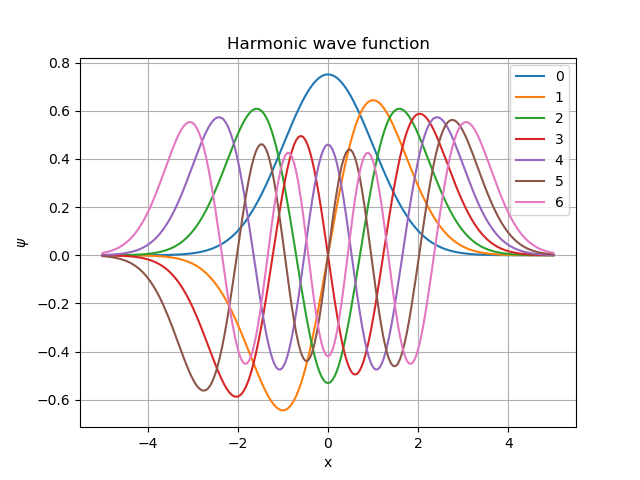
\includegraphics[width=0.9\textwidth]{harmonic_wavefunction}
\end{figure}

\subsection{Spin}

Half-integral spin, e.g. electron or proton. At rest has no orbital rotation, only spin. Spin is angular momentum attached to particle - see (\ref{eq:lx_ly}), (\ref{eq:ly_lz}), and (\ref{eq:lz_lx}). We introduce the Pauli matrices:

$$
\sigma_z = \begin{pmatrix}
1 & 0 \\
0 & -1
\end{pmatrix}
\quad
\sigma_x = \begin{pmatrix}
0 & 1 \\
1 & 0
\end{pmatrix}
\quad
\sigma_z = \begin{pmatrix}
0 & -i \\
i & 0
\end{pmatrix}
$$

and show they satisfy (\ref{eq:lx_ly}), (\ref{eq:ly_lz}), and (\ref{eq:lz_lx}). Actually need $s_i=\frac{\sigma_i}{2}$.

\begin{align*}
[s_x,s_y] =& i s_z \\
[s_y,s_z] =& i s_x\\
[s_z,s_x] =& i s_y\\
J=&L+s\text{, where $J$ is total angular momentum.}
\end{align*}

Eigenvalues of $s_z$ are $\pm \frac{1}{2}$.

Notice that we have integral and half integral spins.

See Figure \ref{fig:degeneracy:hydrogen}. Number of states for each n, 1, 4, 9, 16, ...

For Helium, we can put 2 electrons into ground state; if we try to create an ion with 3 electrons, one goes into next state! Pauli exclusion principle. New property with two values, up and down. Checked with magnetic field.

Pauli's exclusion is a postulate of non-relativistic QM, but a consequence of relativistic QM.

Two kinds of particles: ones that satisfy Pauli, and those that don't.

Identical quantum particles are indistinguishable.

\begin{align*}
\psi(x) =& \braket{x|psi}\\
\psi(x_1,x_2) =& \braket{x_1x_2|psi}\text{, two particles}\\
\psi(x_1,x_2) \rightarrow & \psi(x_2,x_1)\text{, swap using operator $S$}\\
S\ket{x1,x2} =& \ket{x2,x1}\\
S^2 =& 1\text{, and it is unitary.}
\end{align*}

Eigenvalues are $\pm1$.

\section{Fermions: a tale of two minus signs}

Fermions: spin $\frac{1}{2}$ particles, which satisfy Pauli exclusion principle. NB, the 2 electrons in Helium are \textit{entangled}.

Photons don't have an exclusion principle; in fact they have a tendency to congregate.
 
Can we have spin $\frac{1}{2}$ particles that don't obey Pauli exclusion principle? No. Can show this from quantum field theory?

Consider wave function of positions for multiple particles, e.g. $\ket{x_1,x_2,x_3}$. Then $\braket{x_1,...x_n|\psi}=\psi(x_1,...x_n)$

\begin{align*}
\ket{x_1, x_2}=&\ket{x_2, x_1}e^{i\phi}\text{, interchange twice--there are two possibilities}\\
\ket{x_1, x_2}=&+\ket{x_2, x_1}\text{ Bosons}\\
\ket{x_1, x_2}=&-\ket{x_2, x_1}\text{ Fermions}
\end{align*}

NB: sign is not observable.

\begin{align*}
\psi(x_1,x_2)=&-\psi(x_2,x_1) \text{, Fermions}\\
\psi(x_1,x_2)=&-\psi(x_2,x_1) \text{, Bosons}\\
\psi_0(x_1)\psi_0(x_2)& \text{--OK for Bosons but not Fermions}\\
\psi_0(x_1)\psi_1(x_2)& \text{--not OK for Bosons, or Fermions}\\
\psi_0(x_1)\psi_1(x_2)+\psi_0(x_2)\psi_1(x_1)& \text{--OK for Bosons}\\
\psi_0(x_1)\psi_1(x_2)-\psi_0(x_2)\psi_1(x_1)& \text{--OK for Fermions}
\end{align*}

Rotate system by $2\pi$: is there a phase?

\begin{align*}
J_z\ket{\psi} =& -i \frac{\partial \ket{\psi}}{\partial \theta}\\
=& m\ket{\psi} \text{, if eigenvector}\\
\ket{\psi(\theta)} =& e^{im\theta}\ket{\psi(0)}\text{, so $m$ integral or half integral.}
\end{align*}

What if $m$ half integral and we rotate by $2\pi$? We have phase of $-1$, so $\psi$ changes sign.

David Finkelstein. Belt, Deep topological connection between rotation and interchange.

\section{Quantum Field Theory}

In principle covers all natural phenomena except gravity.

\subsection{Review of Harmonic Oscillator}
Imagine many (possibly infinite number) harmonic oscillators.

From (\ref{eq:creation:operator}) and (\ref{eq:annihilation:operator}):
\begin{align*}
a^+_i \triangleq & \frac{P + i \omega x } {\sqrt{2 \omega}} \text{, creation operator} \numberthis \label{eq:creation:operator:i}\\
a^-_i \triangleq & \frac{P - i \omega x } {\sqrt{2 \omega}}\text{, annihilation operator} \numberthis \label{eq:annihilation:operator_i}\\
\end{align*}

Think as each oscillator  as an independent system of degrees of freedom, so operators commute. Using  (\ref{eq:a:comm}), and (\ref{eq:number:operator})

\begin{align*}
[a^+_i,a^+_j] =& 0 \numberthis \label{eq:a:comm_i_plus}\\
[a^-_i,a^-_j] =& 0 \numberthis \label{eq:a:comm_i_minus}\\
[a^-_i,a^+_i] =& \delta_{i,j} \numberthis \label{eq:a:comm_i}\\
H =& \hslash \sum_{i}  \omega_i N_i\text{, where $N_i$ are known as occupation numbers.}
\end{align*}
We're ignoring ground state energy.

One basis of states is $\ket{n_1,n_2,n_3,...}$.

\begin{thm}
	$a^+\ket{n}=\sqrt{n+1}\ket{n+1}$
\end{thm} 

\begin{proof}
	\begin{align*}
	a^+\ket{n}=&c_n\ket{n+1}\\
	\bra{n}a^-=&c_n\bra{n+1}\text{, assume real}\\
	\braket{n|a^-a^+|n}=&c_n^2\text{, normalization!}\\
	=& \braket{n|a^+a^-+1|n}\text{, using commutator}\\
	=& \braket{n|N+1|n}\\
	=&n+1
	\end{align*}
\end{proof}

\begin{cor}
	$a^-\ket{n}=\sqrt{n}\ket{n-1}$
\end{cor}


$a_i^+\ket{n_1,n_2,.....}=\sqrt{n_i+1}\ket{n_1,n_2,...n_i+1,...}$

\subsection{Quantum Field Theory of Bosons}

Fields are functions of position. $\psi(x)$ not observable; we observe position, momentum, etc, but not $\psi$. $psi(x_1,x_2,...x_15)$ function of many positions.

\begin{itemize}
	\item $\Psi$ is an observable, e.g. magnetic field, so an operator.
	\item $Psi$ function of one position
	\item $Psi$ describes any number of particles.
\end{itemize}


Consider one particle in a box, and think about energy eigenstates. Wave function $\psi_1(x)$ is sine (lowest energy level). Next $\psi_2(x)$ has one node, with higher energy.

Now many particles (bosons), some in first energy level, some in second,...$\ket{n1,n2,n3,...}$> Now we invent operators as in (\ref{eq:a:comm_i_plus}) - (\ref{eq:a:comm_i}) to create and remove particles. NB $\set{1,2,3,...}$ are states $\set{n_i}$ occupation numbers.

\begin{align*}
(a^+a^-)\ket{n}=&(a^-a^+-1)\ket{n}\\
=&\sqrt(n+1)a^-\ket{n+1}-\ket{n}\\
=&(n+1)\ket{n}-\ket{n}\\
=&n\ket{n}
\end{align*}

NB: we are \text{ defining} creation and annihilation operators. Don't ask why for a definition, ask why it is useful. E.g. creation lets us create a photon. We want to study system with variable number of photons.

Vacuum is state that is annihilated by $a^-$ -- $\ket{0,0,0,....}$.

Denote energy by $\omega_i$ for state $i$. 

\begin{align*}
E =& \sum_{i} n_i \omega_i\\
=& \sum_{i} \omega_a a^+_i a^-_i 
\end{align*}

We'll consider free particles--no interactions.

Whey can we ignore ground-state energy? Because constants commute with everything. 

Quantum fields theory is a book-keeping device for particles.

$\Psi(x)$ -- an operator that is a function of position--Fock Space

\begin{align*}
\Psi(x)\triangleq&\sum_{i}a^-_i\psi_i(x)\text{, not Hermitean, so conjugate is}\\
\Psi^\dagger(x)=&\sum_{i}a^+_i\psi_i^*(x)\\
\Psi(x)+\Psi^\dagger \text{ is}&\text{ Hermitean}
\end{align*}

What if we apply to vacuum? $\Psi(x)$ annihilates it--what about $\Psi(x)^\dagger$.

\begin{align*}
\sum_{i} \ket{i} \bra{i} =& I \text{, sum over states with $\psi_i$}\\
\sum_{i} \ket{i} \braket{i|X} =& \ket{X}\\
\psi^*_i(x)\underbrace{\ket{i}}_\text{one particle with state $i$} =& \ket{X}\text{, but}\\
\ket{i} =& a^+_i\ket{0} \text{, whence}\\
\psi^*_i(x) a^+_i\ket{0}=&\ket{x}\\
\Psi^\dagger(x) \ket{0} =& \ket{x}\text{ so $\Psi^\dagger(x)$ creates a particle at $x$.}
\end{align*}

\begin{itemize}
	\item $a^+_i$ creates a particle in state $i$.
	\item $\Psi^\dagger(x)$  creates a particle at position $x$.
	\item $a^-_i$ annihilates a particle in state $i$, or gives zero.
	\item $\Psi(x)$  annihilates a particle at position $x$, or gives zero.
\end{itemize}

There is a separate field for each Boson.

Add vacuum to a state, we get probability of 0.5 of vacuum. It is not the same as zero. Vacuum has length of 1!

Let's add two particles, at $x$ and $y$. 
 
\begin{align*}
\Psi(y)\Psi(x)\ket{0} =& \ket{y,x}\\
\Psi(x)\Psi(y)\ket{0} =& \ket{x,y} \text{, but from (\ref {eq:a:comm_i_plus})}\\
\Psi(y)\Psi(x) =& \Psi(x)\Psi(y) \text{, so}\\
\ket{x,y} =& \ket{y,x} \text{, which is what we expect for Bosons.} 
\end{align*}

We can handle situation where number of particles is a random variable: a laser wave is a superposition.

\section{Quantum Field Theory II}

Can start with particles and see why they can be described by fields, or start with fields and quantize. Starting with particles we can use fields to handle variable numbers. Normalization $\int \psi^*(x) \psi(x) dx=1$ gives \textit{number of particles}.

Given an orthonormal basis:
\begin{align*}
\sum_{i} \ket{i} \bra{i} =& I \text{, "Resolution of the Identity"}\numberthis \label{eq:resolution:identity}\\
\braket{y|x}=& \sum_{i} \braket{y|i} \braket{i|x}\\
\delta(x-y)=& \sum_{i} \psi_i(y) \psi^*_i(x)\text{, for any set of eigenvectors of Hermitan operator.}
\end{align*}

Can characterize multi-particle system by $\ket{n_1, n_2,...n_i,...}$. We want to increase and decrease occupation numbers, so introduce creation and annihilation operators.

\begin{itemize}
	\item $a^+_i=a^\dagger_i$
	\item $a^-_i=a_i$
\end{itemize} 

Introduce field operator
\begin{align*}
\Psi(x) \triangleq & \sum_{i} a_i \psi_i(x) \text{, would be Fourier if sine/cosine waves}\\
\Psi^\dagger(x) =& \sum_{i} a^\dagger \psi^*_i(x)\\
\Psi(x) + \Psi^\dagger(x) \text{ is}& \text{ Hermitean (observable)}\\
\frac{\Psi(x) - \Psi^\dagger(x)}{i} \text{ is}& \text{ Hermitean (observable)}
\end{align*}

Vacuum: $\ket{0} = \ket{0,0,0,.....}$.

\begin{align*}
\ket{x}=&\sum_{i}\ket{i}\braket{i|x}\text{, from (\ref{eq:resolution:identity})}\\
=& \sum_i \psi^*_i(x)a^\dagger_i\ket{0}\\
=& \Psi^\dagger(x) \ket{0}\text{, creation operator at a point.}
\end{align*} 

Consider the following operator:
\begin{align*}
\int dx \Psi^\dagger(x) \Psi(x)=&\int dx \sum_{i,j}a^+_i\psi_i^*(x) a_j\psi_j(x)\\
=&\sum_{i,j} a^+_i a_j \int dx \psi_i^*(x) \psi_j(x)\\
=&\sum_{i,j} a^+_i a_j \delta_{i,j}\\
=&\sum_i a^+_i a_i\\
=&\sum_i N_i\text{, operator representing total number of particles.}
\end{align*}

To make energy finite, total number of particles must be finite. $\Psi^\dagger(x) \Psi(x)$ represents particle density.

We now calculate the total energy.

\begin{align*}
E =& \sum_{i} N_i \omega_i\\
=& \sum_{i} a^\dagger_i a_i \omega_i
\end{align*}

We determine $\omega_i$ from eigenvalues of Schr\"odinger equation (ignoring interactions):
\begin{align*}
H \psi_i =& \omega_i \psi_i\\
\big[\frac{p^2}{2m} + V(x)\big]\psi_i(x)=& \omega_i \psi_i(x)\\
\big[-\frac{\nabla^2}{2m} + V(x)\big]\psi_i(x)=& \omega_i \psi_i(x)
\end{align*}

Guess solution
\begin{align*}
E=&\int dx \underbrace{\Psi^\dagger(x) \big[-\frac{\nabla^2}{2m} + V(x)\big] \Psi(x)}_\text{energy density} \\
=& \int dx \sum_{i,j}a^+_i\psi_i^*(x)\big[-\frac{\nabla^2}{2m} + V(x)\big]\psi_j(x)a^-_j\\
=& \int dx \sum_{i,j} a^+_i a^-_j \psi_i^*(x) \omega_j \psi_j(x)\\
=&  \sum_{i,j} a^+_i a^-_j \delta_{i,j} \omega_j
\end{align*}

Behaves like classical theory if the number of particles is very large.


\section {Second Quantization}

\section{Quantum field Hamiltonian}

\section{Fermions and the Dirac equation}

\end{document}
